\documentclass[conference]{IEEEtran}
\usepackage{cite}
\usepackage{amsmath,amssymb}
\usepackage{graphicx}
\graphicspath{{figs/}}
\usepackage{booktabs}
\usepackage[hidelinks]{hyperref}

\begin{document}

\title{Graph Neural Network Surrogates for a Coupled Heat-Conduction and
Pyrolysis Solver in Thermal Protection System Design}

\author{\IEEEauthorblockN{Grey Goodwin}
\IEEEauthorblockA{University of Kentucky \\
Lexington, KY, USA \\
grey.goodwin@uky.edu}}

\maketitle

\begin{abstract}
% DRAFT abstract from the white paper; tighten to ~150-200 words for IEEE.
Thermal protection system (TPS) design relies on repeated evaluation of an
expensive physics solver that resolves heat conduction, pyrolysis,
pyrolysis-gas transport, and aerothermal surface chemistry. We present early work
toward a graph neural network (GNN) surrogate that learns the per-step evolution
of a 1D heat-shield pyrolysis solver. As a foundation, we port a trusted
Fortran reference solver to Python and verify it against the original by comparing
thermocouple and density outputs. We test two cases of increasing difficulty: a
gas-off conduction--pyrolysis case matches to machine precision, and a full
gas-plus-aerothermal case matches to 0.064~K. Training on data from the validated solver, a
per-cell message-passing GNN reproduces a held-out heating scenario over a full
60~s rollout to a mean error of 7.6~K and tracks the pyrolysis front to within a
fraction of a millimeter. On the full gas case a purely learned predictor diverges on held-out forcings.
Structuring the known physics into the surrogate fixes this. We fix the
conduction rate and the Arrhenius pyrolysis to the reference solver and let the
network learn only the residual gas coupling, inside an update that cannot blow
up by construction. The resulting surrogate reproduces a held-out gas case over a
full 120~s rollout to a mean error of 25~K, tracks the char front to about a
millimeter, and runs about ten times faster than the Python solver and about twice
as fast as the reference Fortran solver. A stiff coupled problem needs its known
physics built into the surrogate, where the gas-off case did not.
\end{abstract}

\begin{IEEEkeywords}
graph neural networks, surrogate models, thermal protection systems, pyrolysis,
scientific machine learning
\end{IEEEkeywords}

\section{Introduction}
% 1.1 TPS / heat-shield design problem
% 1.2 + 1.3 cost bottleneck and the surrogate response (CITE motivation \cite{...})
% 1.4 contribution and scope
% 1.5 relation to prior bead/Sod work (CITE own work \cite{...})
Thermal protection systems (TPS) shield a vehicle from the intense aerothermal
heating of atmospheric entry. Designing one means choosing a material and a
thickness that keep the structure beneath the heat shield below its temperature
limit while adding as little mass as possible~\cite{mazzaracchio2010,lu2024}. The
governing physics is a coupled, strongly nonlinear problem: heat conducts into the
material, the material pyrolyzes (chemically decomposes) as it heats, the
pyrolysis gas percolates out through the charring solid, and the exposed surface
exchanges energy with the hot boundary layer~\cite{pan2023,mazzaracchio2010}.

A solver accurate enough for design is expensive to run~\cite{queipo2005}.
Detailed material-response codes, and especially simulations that couple the
material response to a CFD boundary layer, are costly per run~\cite{pan2023}. Design multiplies that cost. Sizing, optimization, and uncertainty studies each
call the solver many times over~\cite{pan2023,mazzaracchio2010,lu2024}. The per-run cost
multiplied by the number of calls is the bottleneck a surrogate targets. The
response we pursue is a machine-learned surrogate trained on data from a trusted
reference solver, so a design loop can replace most solver calls with fast
surrogate evaluations~\cite{queipo2005,kochkov2021,brandstetter2022}. The 1D reference solver used here is
itself inexpensive, only a few minutes per run, so we treat it as a tractable,
fully validated testbed for developing the surrogate method. The speed payoff is
intended for the higher-fidelity, higher-dimensional solvers this method should
extend to.

We use a graph neural network for the surrogate because the discretized solver is
naturally a graph. The mesh cells are nodes and adjacent cells are connected by
edges~\cite{sanchez2020learning,meshgraphnets}. A GNN that shares its weights
across all cells is mesh-native and, in principle, applies to a mesh of any
size~\cite{meshgraphnets,brandstetter2022}, which is the property we ultimately want for a
tool that must run at varying resolutions.

This paper reports three things. First, a faithful Python re-implementation of the
reference Fortran solver, verified against the original to machine precision on
the conduction--pyrolysis case and to a small fraction of a kelvin on the full
multi-physics case. Second, a working surrogate for the conduction--pyrolysis
case, accurate over a full rollout on a held-out scenario. Third, a working
surrogate for the full gas case, built by structuring the known physics into the
model. A purely learned model diverges there. Fixing the conduction and pyrolysis
physics to the reference solver, bounding each update so it cannot blow up, and
learning only the gas coupling yields a surrogate that is accurate over a held-out
rollout and faster than the solver. The gas case shows that a stiff coupled
problem needs its known physics built in, where the simpler gas-off case did not.

\section{Reference Solver}
The reference is a 1D finite-volume heat-shield code written in Fortran. It models,
in one spatial dimension through the thickness of the slab:
\begin{itemize}
  \item \textbf{Heat conduction} with temperature-dependent and
  char-state-dependent material properties.
  \item \textbf{Pyrolysis}, the heat-driven decomposition of the solid, modeled as
  a set of Arrhenius reactions that consume reactive species and release gas.
  \item \textbf{Pyrolysis-gas transport} through the porous char (Darcy flow plus
  advection), which carries energy and couples back into the temperature field.
  \item \textbf{An aerothermal surface boundary}, including a B-prime
  surface-chemistry table (a precomputed ablation-thermochemistry lookup), a
  blowing correction, and a wall-enthalpy balance, representing the interaction
  with the hot boundary layer.
\end{itemize}
The solver advances the standard in-depth energy equation for a charring ablator,
a conduction-diffusion balance
\begin{equation}
\rho\, c_p\, \frac{\partial T}{\partial t}
  = \frac{\partial}{\partial x}\!\left(k\, \frac{\partial T}{\partial x}\right)
  + (\text{pyrolysis and gas source terms}),
\end{equation}
where $T$ is temperature, $\rho$ the density, $c_p$ the specific heat, $k$ the
thermal conductivity, $x$ the depth coordinate, and $t$ time. The properties
$\rho$, $c_p$, and $k$ all depend on temperature and char state, so the equation
is nonlinear. The source terms collect the pyrolysis energy and the enthalpy
transported by the gas, and we do not expand them here. The equation is
discretized on a finite-volume mesh. Each cell carries a temperature and a set of
species densities. The conduction term is evaluated from temperature differences
across cell faces, and the pyrolysis term advances each species by a closed-form
Arrhenius update. Material properties are blended between virgin and char states by
a char-progress variable derived from the local density.

Three reference cases ship with the code and are used throughout: \texttt{aw1}, a
conduction-plus-pyrolysis case with a prescribed wall-temperature history and the
gas physics off; and \texttt{aw2\_tc21} and \texttt{aw2\_tc22}, which add the full
gas and aerothermal boundary. As shipped, \texttt{aw2\_tc22} is configured
identically to \texttt{aw2\_tc21}.

\section{Methodology}
\subsection{Python Port}
The solver was re-implemented in Python one physics module at a time: grid and
geometry setup, mixture properties, the Arrhenius pyrolysis update, the gas solve,
and the aerothermal boundary. Where a coding choice affected the numerical result,
the Python deliberately matched the Fortran. The thermocouple sampling in
particular was rewritten to mirror the reference probe-sampling routine, clamping
to the face value at domain boundaries and reconstructing it by interpolation in
the interior. Three details proved to matter for agreement. First, thermocouple positions are
given as depth from the right wall. Second, the face density used to evaluate the
face conductivity is the pre-pyrolysis density, matching the Fortran update order.
Third, output is written before the physics step, matching the reference
time-offset convention.

\subsection{Verification}
Verification is done by direct column-by-column comparison against the Fortran
output from a run with identical configuration. For every output column (time,
each thermocouple temperature, and each density), we report the maximum absolute,
mean absolute, and maximum relative error across the run. This is a strict test:
it compares the full time history at every recorded probe, not just a summary
statistic.

\subsection{Training-Data Generation}
Once verified, the Python solver generates the training data. Each run records the
full per-cell field over time (temperature, bulk density, the per-species
densities, and, in gas runs, the gas pressure and mass flux), including the two
ghost cells at the domain ends that carry the boundary forcing. A single recorded
trajectory can later be turned into training pairs at any time-step spacing without
re-running the solver. The first dataset varies the boundary forcing, a sweep of
wall-temperature histories, on the fast gas-off \texttt{aw1} case.

\subsection{GNN Architecture}
The surrogate is a per-cell message-passing network. Each finite-volume cell is a
node carrying the state vector $[T,\rho,\rho_i,\text{porosity}]$. Adjacent cells
are joined by edges whose features are relative: the difference between the
neighbor's state and the cell's own, together with the cell spacing. This relative
encoding mirrors the physics, since the conduction flux between two cells depends
on their temperature difference and their spacing. A forward step encodes the node
and edge features with small multilayer perceptrons, performs one round of message
passing (each cell aggregates the encoded messages from its left and right
neighbors and updates its hidden state), and decodes a predicted change in the
cell's state, which is added to the current state and rolled forward in time. A
single message-passing round matches the nearest-neighbor reach of the conduction
stencil, and weight sharing across cells lets the same model apply to a mesh of any
length. The model predicts only the independent degrees of freedom, temperature and
the per-species densities; bulk density and porosity are derived from them. Training
minimizes the error of a short multi-step rollout rather than a single step, which
controls the accumulation of error over a long rollout (Section~\ref{sec:aw1acc}).

\begin{figure}[t]
  \centering
  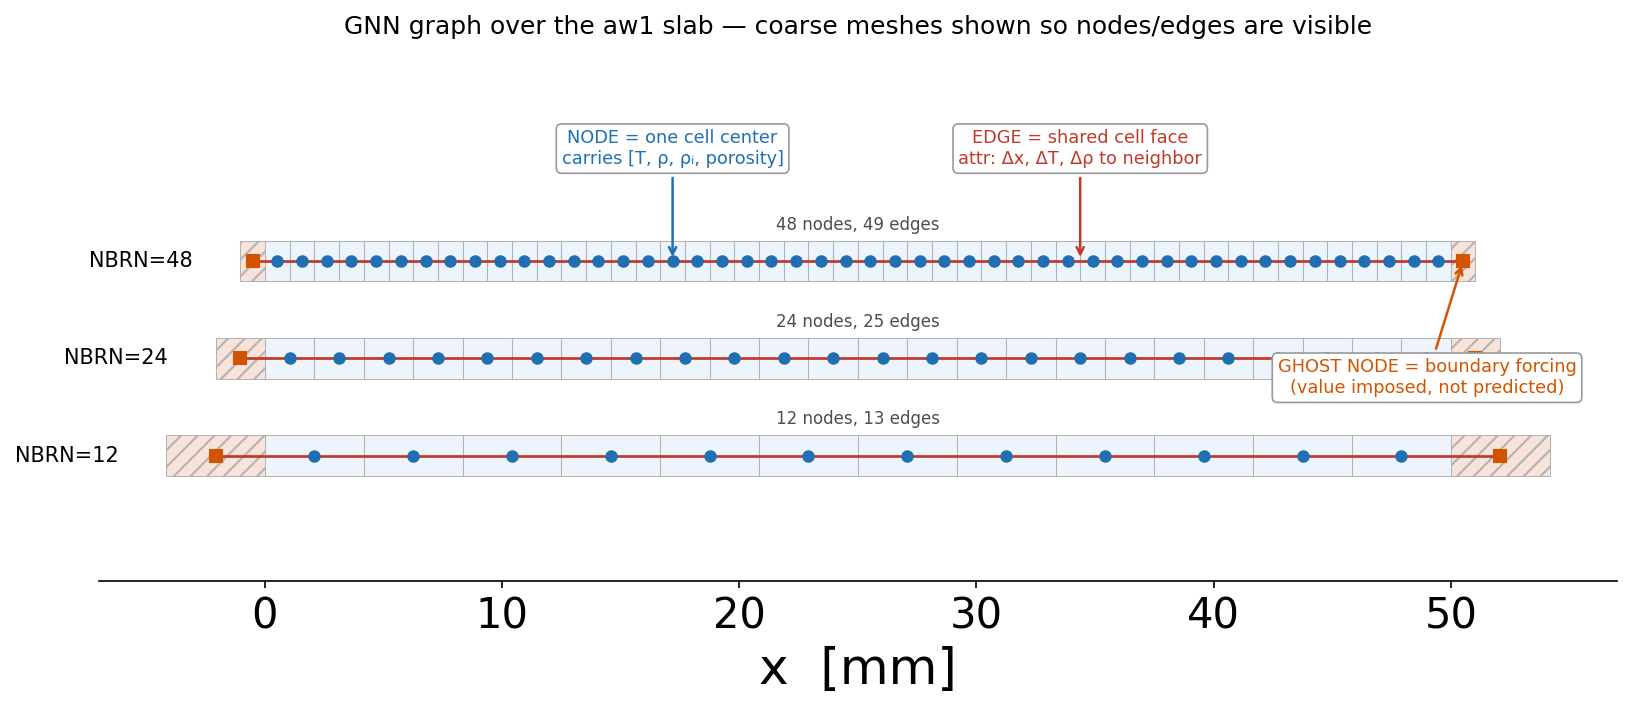
\includegraphics[width=\columnwidth]{graph.png}
  \caption{The mesh as a graph: each finite-volume cell is a node carrying
  $[T,\rho,\rho_i,\text{porosity}]$; edges join neighboring cells with relative
  features (neighbor-minus-self state and the cell spacing $\Delta x$). Ghost
  nodes at the ends impose the boundary forcing. Weights are shared across all
  cells. (Coarse meshes shown for legibility.)}
  \label{fig:graph}
\end{figure}

\subsection{Conservative Flux-Form Variant}
The gas-case failure (Section~\ref{sec:aw2}) motivates a second output
formulation. Rather than predicting a per-cell state change directly, the model
predicts a flux on each cell face and forms the change as the net flux across the
cell's two faces plus a local source,
\begin{equation}
\Delta_i = \left(F_{i-1/2} - F_{i+1/2}\right) + S_i ,
\end{equation}
where $F_{i\pm1/2}$ are the face fluxes and $S_i$ is a local source. The face flux
is constructed antisymmetric, $F(a,b) = -F(b,a)$, giving two properties by
construction: (i)~conservation, since whatever leaves a cell across a face enters
its neighbor; and (ii)~a zero baseline, since a uniform field yields zero face
flux, so quiescent cells receive no transport change and the per-step bias cannot
arise. Change not driven by a neighbor gradient, the local pyrolysis source, is
carried by $S_i$. The flux and source are produced by the same weight-shared
message-passing network, and the change is decoded with no constant offset so the
zero baseline survives. This is the conservative, divergence-form construction
used for learned solvers~\cite{brandstetter2022,kochkov2021}.

\subsection{Physics-Informed Conductance Form}
\label{sec:cond}
The flux-form removes the divergence but still asks the network to learn the
conduction and pyrolysis rates from short rollouts, which it does poorly for the
stiff gas case (Section~\ref{sec:physcond}). The final formulation builds the
known physics in and narrows what is learned.

The face flux is written as a conductance times the state difference across the
face, $F_{i+1/2} = D\,(s_i - s_{i+1})$ with $D \ge 0$. The conductance on each
face is capped at one over the node degree, so a cell's update is a weighted
average of itself and its neighbors with non-negative weights that sum to one.
Such an update obeys a discrete maximum principle. The new value lies between the
smallest and largest of the neighboring values, so the field cannot grow beyond
its surroundings and the rollout is stable at any step size. This is a stronger
guarantee than the flux-form's zero baseline, which prevents drift but not
overshoot.

Two rates that the flux-form left to the network are instead fixed to the
reference solver. First, the conduction rate $D$ for temperature is set to the
diffusion number measured from the solver, not learned, because a short rollout is
blind to the slow accumulation of a diffusion error and consistently
under-diffuses. Second, the pyrolysis source is the solver's own per-species
Arrhenius update, evaluated directly rather than approximated by a learned
function. The network is then responsible only for the coupling from the gas state
to the total decomposition rate, a small number of parameters. Because a single
bounded update moves heat only to the nearest neighbor, one data step is advanced
as several bounded sub-steps with the boundary forcing held fixed across them,
which lets the thermal front travel the physical distance of one super-step while
keeping the maximum-principle guarantee.

\section{Results}
\subsection{Port Validation}
On \texttt{aw1} (conduction plus pyrolysis), all fifteen output columns match the
Fortran output to approximately $10^{-8}$, machine precision, including every
interior thermocouple: the conduction and pyrolysis port is exact. On
\texttt{aw2\_tc21} (full gas plus aerothermal), with the gas physics enabled and
compared against the same-configuration Fortran output, agreement is summarized in
Table~\ref{tab:val}.
\begin{table}[t]
\caption{Port validation against the Fortran reference (\texttt{aw2\_tc21}).}
\label{tab:val}
\centering
\begin{tabular}{ll}
\toprule
Quantity & Agreement \\
\midrule
All temperature columns & max 0.064~K, mean $\sim$$4\times10^{-4}$~K \\
Hot aerothermal surface & 0.06~K \\
Densities & $\sim$$10^{-3}$ to $10^{-9}$ \\
Time, cold back face & bit-exact \\
\bottomrule
\end{tabular}
\end{table}

During verification, an apparent early interior drift and a roughly 37.7~K
back-face offset both proved to be artifacts of how the thermocouples were sampled,
not numerical error; both vanished once the probe sampling matched the reference
routine. Comparing two temperature fields through a sampling layer can manufacture
a discrepancy that is not present in the physics itself. As shipped,
\texttt{aw2\_tc22} is byte-for-byte identical in configuration to
\texttt{aw2\_tc21} and so adds no independent validation condition.

\subsection{Surrogate Accuracy (aw1)}
\label{sec:aw1acc}
Trained on solver-generated trajectories, the surrogate is rolled forward on its
own predictions over a held-out \texttt{aw1} heating scenario (gas off) for the
full 60~s, with the known boundary forcing re-imposed each step. The mean rollout
error is 7.6~K, roughly half a percent to one percent of the 298 to 1500~K field,
and the surrogate tracks the char and pyrolysis front to within a fraction of a
millimeter (Fig.~\ref{fig:aw1rollout}). Reaching this required training on
multi-step rollouts rather than single steps: a single-step-trained model is
accurate for one prediction but accumulates error and drifts once rolled forward
freely, and the end-of-trajectory error fell from several hundred kelvin to tens of
kelvin under a multi-step rollout loss. This error-accumulation behavior, and its
mitigation by noise injection and multi-step training, are well documented for
learned simulators~\cite{sanchez2020learning,brandstetter2022}.

\begin{figure*}[t]
  \centering
  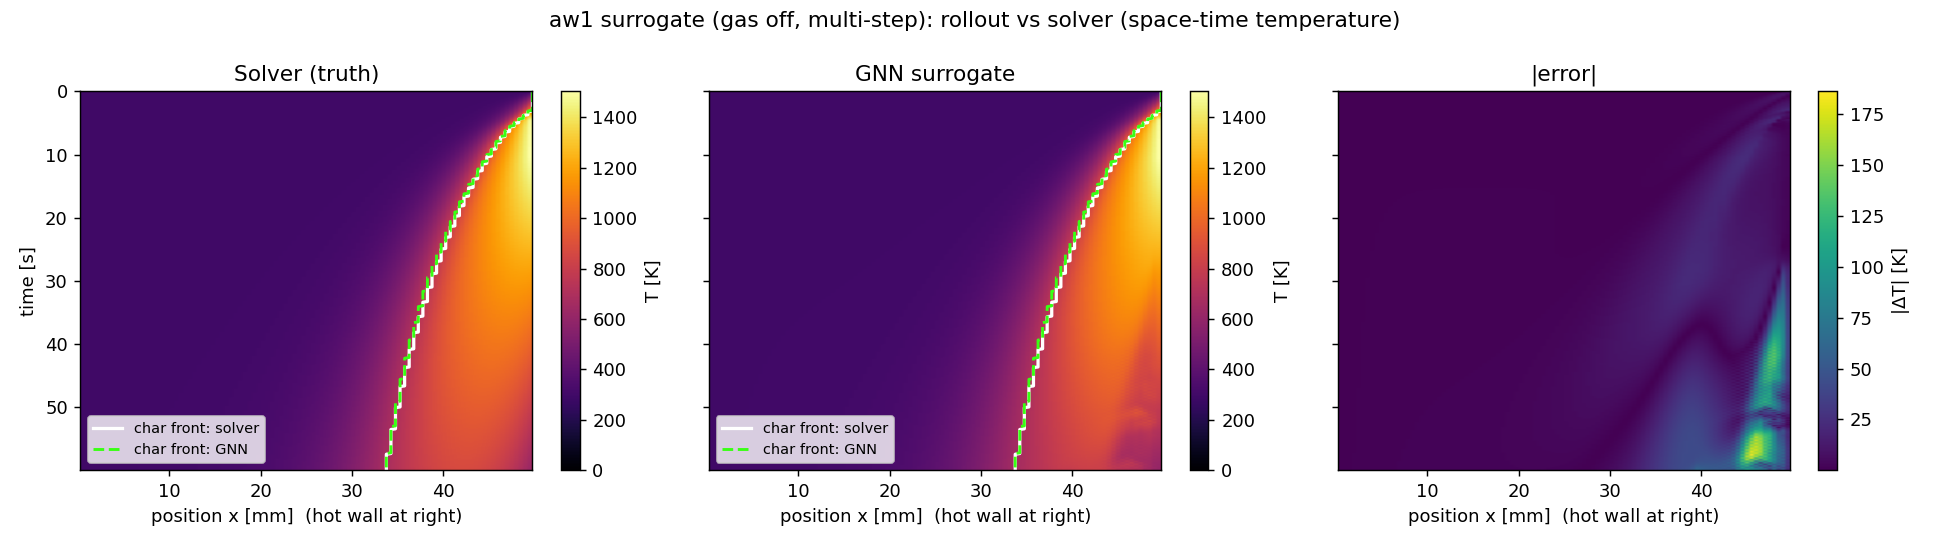
\includegraphics[width=\textwidth]{aw1_rollout_spacetime.png}
  \caption{aw1 surrogate rollout (gas off), space-time temperature. Solver truth
  (left), GNN surrogate (center), absolute error (right). The white and green
  char-front curves on the two temperature panels nearly coincide, so the surrogate
  tracks the pyrolysis front. Mean rollout error 7.6~K over the full 60~s. The
  surrogate field is visually indistinguishable from the solver and the error is
  small everywhere.}
  \label{fig:aw1rollout}
\end{figure*}

\subsection{Gas Case (aw2): Why a Purely Learned Model Fails}
\label{sec:aw2}
Extending the direct per-cell surrogate to the full gas-plus-aerothermal case does
not produce a usable model, and the way it fails is informative. It also guides the
formulation that eventually works (Section~\ref{sec:physcond}). Trained and rolled out on the
same forcing, it converges to a bounded error of about 625~K. The proper test is
harder. Training on a sweep of eight flux histories and rolling out on an unseen
one, the model diverges to several thousand kelvin. The in-sample result was
optimistic. The model largely fits the one trajectory it is evaluated on and does
not generalize across forcings. The divergence is not subtle. On the held-out case
the predicted field runs past 100{,}000~K while the solver stays under 1700~K
(Fig.~\ref{fig:contrast}, center).

The cause is temporal, not spatial (Fig.~\ref{fig:why}). Per cell, \texttt{aw2}
is no steeper than \texttt{aw1}, since its finer mesh spreads the gradient over
more cells. What differs is the rate of change per step. The \texttt{aw2} surface,
driven by a square-pulse aerothermal flux, heats from about 300~K to over 1500~K in
roughly one second. It therefore moves hundreds of kelvin in a single coarse
super-step, against tens of kelvin for \texttt{aw1}, and a fixed super-step cannot
track that. This is a known difficulty for learned solvers. Physics-informed
networks fail in the same way at high-gradient or discontinuous boundaries, where
local errors accumulate over time and corrupt the global field~\cite{cao2026}.
We tried several fixes within this formulation and none closed the held-out gap. A
time-step-aware adaptive schedule, with fine steps near the transient and coarse
steps on the plateau, bounds the in-sample rollout but not the held-out one. Adding
more training trajectories, treating the gas state as a known input, and widening
the stencil did not help either. The reference solver was verified sound on this
case, so the failure is the surrogate's, not the data's. This bounds where a
per-cell state-delta GNN of this kind applies and motivates the conservative
formulation of Section~\ref{sec:flux}.

\begin{figure*}[t]
  \centering
  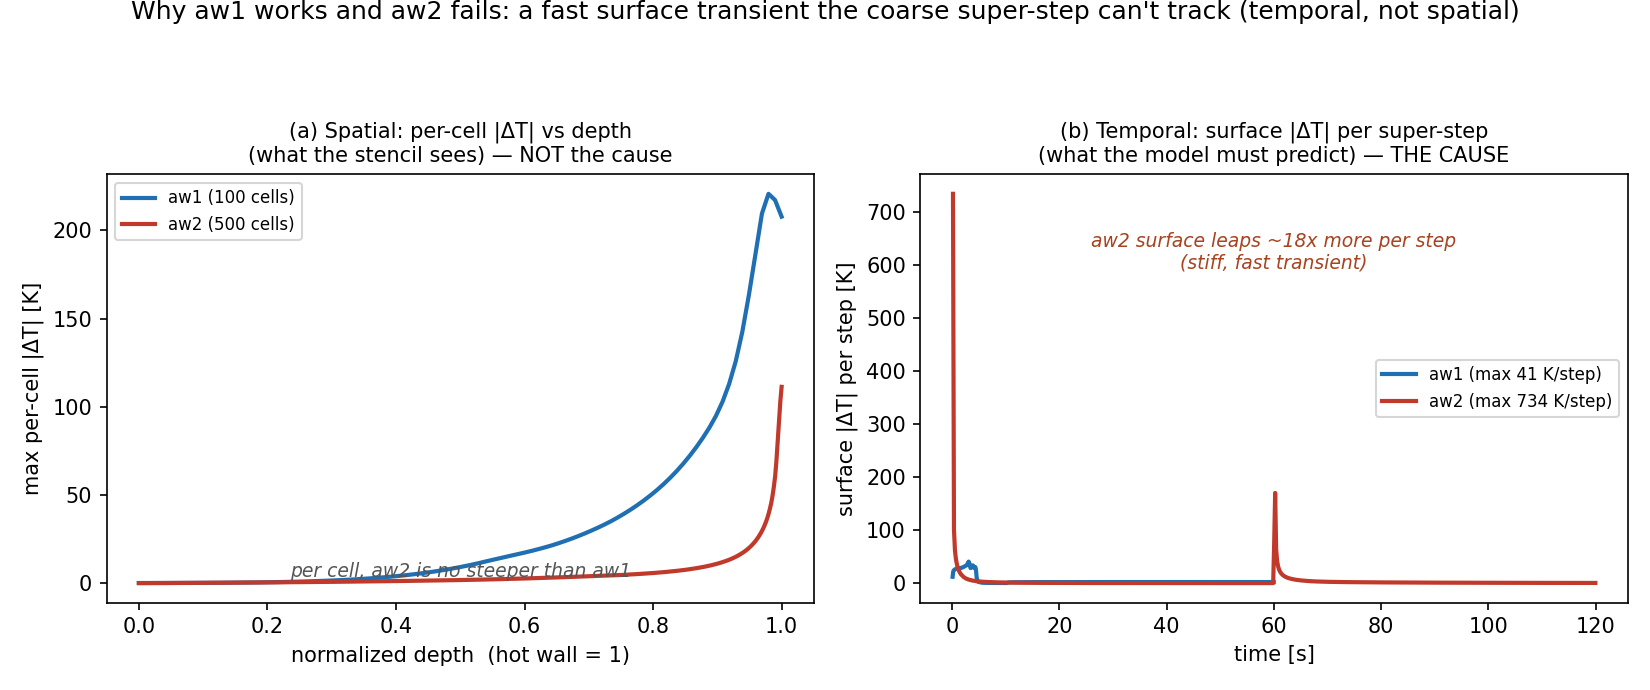
\includegraphics[width=\textwidth]{why_aw1_aw2.png}
  \caption{Why aw2 fails and aw1 does not, and why the cause is temporal not
  spatial. (a) Per-cell spatial $|\Delta T|$: aw2 is no steeper than aw1.
  (b) Per-super-step surface $|\Delta T|$: aw2 leaps $\sim$18$\times$ more
  (734 vs 41~K) under the square-pulse aerothermal flux, which a fixed coarse
  super-step cannot track.}
  \label{fig:why}
\end{figure*}


\subsection{Conservative Flux-Form Removes the Divergence}
\label{sec:flux}
The flux-form variant of the preceding section was trained on the same
eight-forcing \texttt{aw2} dataset as the direct model, with identical
single-step training and the gas state held from truth so
the test isolates the thermal and chemical rollout. The two models differ only in
their output. Both were rolled out on a held-out forcing, not among the eight
training cases, recorded at the training cadence so the comparison carries no
time-step mismatch (Table~\ref{tab:flux}, Fig.~\ref{fig:fluxcompare}).

\begin{table}[t]
\caption{Held-out \texttt{aw2} rollout: mean interior $T$ error, direct vs.\
conservative flux-form.}
\label{tab:flux}
\centering
\begin{tabular}{lrr}
\toprule
 & Direct & Flux-form (best run) \\
\midrule
Over the full 120~s rollout & 8755~K & 121~K \\
At the end of the rollout    & 25434~K & 104~K \\
End-of-rollout maximum       & 38359~K & 312~K \\
\bottomrule
\end{tabular}
\end{table}

\begin{figure}[t]
  \centering
  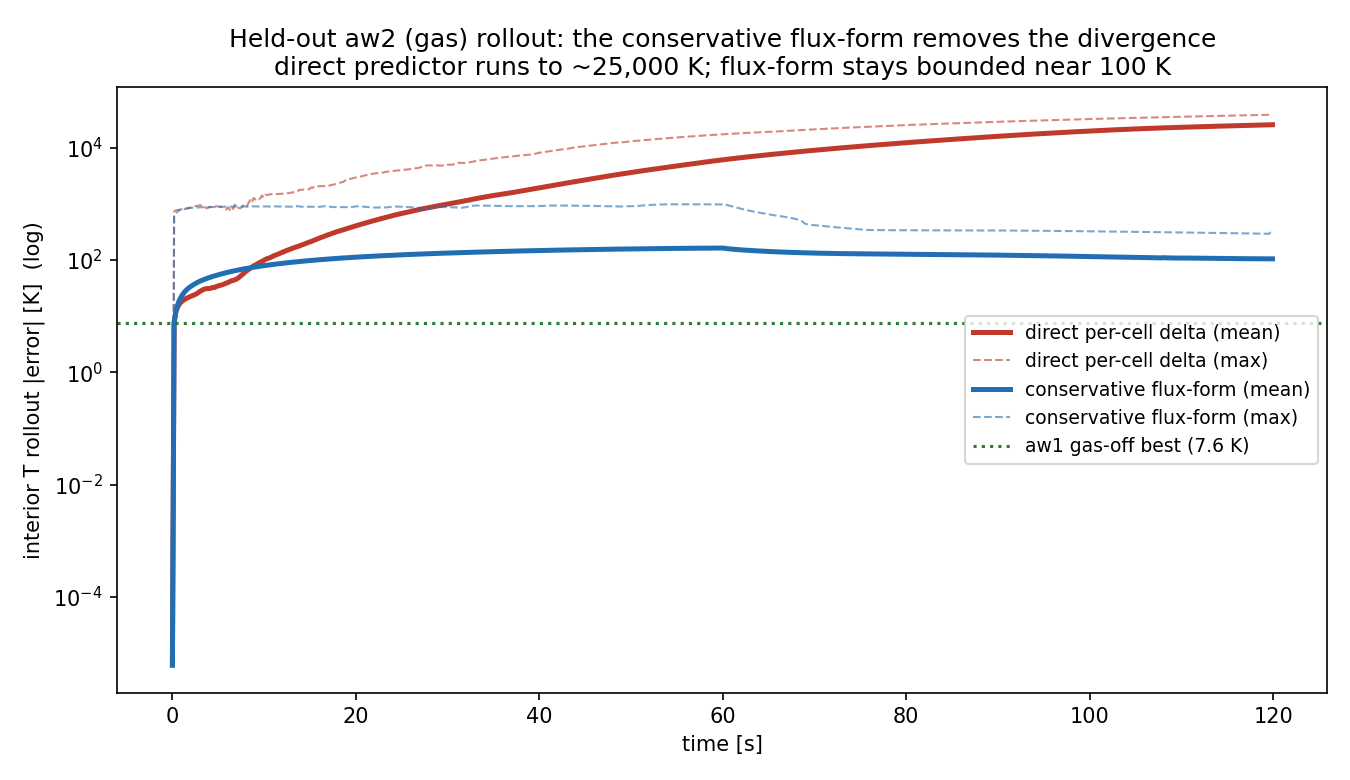
\includegraphics[width=\columnwidth]{flux_aw2_compare.png}
  \caption{Held-out \texttt{aw2} rollout error vs.\ time (log scale). The direct
  per-cell-delta model diverges past $10^4$~K; the conservative flux-form stays
  bounded near 100~K on the unseen forcing.}
  \label{fig:fluxcompare}
\end{figure}

The direct model diverges to $\sim$25{,}000~K by the end of the rollout at this
coarse recording cadence, and further still at the fine cadence of
Fig.~\ref{fig:contrast}. Either way it is the failure diagnosed in
Section~\ref{sec:aw2}. The flux-form, in its best run, stays bounded
near 100--160~K throughout, roughly a $240\times$ reduction in end error, on a
forcing it did not see in training. The conservative formulation removes the
catastrophic divergence. The quiescent-cell bias that drove the direct model past
$25{,}000$~K cannot arise by construction, and that structural fix is the result
that holds.

The residual error is neither small nor consistent run to run. Characterizing it
honestly needs a distribution, since training is unseeded and closed-loop
stability is sensitive to initialization. We trained eight seeds on each of two
datasets and rolled each out on the same held-out forcing (Table~\ref{tab:seeds}).
The single-step loss is nearly identical across seeds, so the variation is not in
how well each learns the one-step map but in closed-loop stability. Composing that
map over hundreds of steps amplifies or damps small errors depending on the
learned local gain, and the under-constrained post-cutoff cooldown sits on the
knife edge. Every run is bounded through heating and the flux cutoff; the
divergence, when it occurs, is in the long cooldown tail.

\begin{table}[t]
\caption{Held-out \texttt{aw2} over eight random seeds, eight vs.\ twenty-four
training forcings: interior $T$ error and char-front fidelity. More data tightens
the temperature mean but does not make a faithful char front the norm.}
\label{tab:seeds}
\centering
\begin{tabular}{lrr}
\toprule
 & Eight & Twenty-four \\
 & forcings & forcings \\
\midrule
Mean $T$ error across seeds       & 850~K       & 419~K \\
$T$ error range (min--max)        & 155--2312~K & 203--543~K \\
Seeds with mean $T > 1000$~K      & 3 of 8      & 0 of 8 \\
Char-front error, best seed       & 0.8~mm      & 1.5~mm \\
Seeds tracking front $<4$~mm      & 2 of 8      & 3 of 8 \\
Seeds false-charring to back face & 5 of 8      & 5 of 8 \\
\bottomrule
\end{tabular}
\end{table}

Two things follow. First, more data removes the worst failures: the eight-forcing
model diverges outright in three of eight seeds (to tens of thousands of kelvin),
while the twenty-four-forcing model keeps every seed in 203--543~K. Second, and
decisive for the verdict, a low mean error does not mean a faithful field, and
none of these models produces one. The mean is taken over 500 cells, mostly the
cool interior that is trivial to predict, so it flatters the model. The
char-front depth, a design-relevant quantity rather than a domain average, makes
this concrete (Table~\ref{tab:seeds}). Only two of eight eight-forcing seeds and
three of eight twenty-four-forcing seeds track the front to within a few
millimeters, while in five of eight either way the model reports the entire slab
charred to the back face. A faithful char front is the exception at both sizes;
more data tightens the mean but does not fix it. Inspecting the rollout tells a
different story than the mean. The best eight-forcing run (mean
104~K) is bounded and qualitatively right, the surface heating and cooling on the
correct schedule and the char front within a few millimeters of the solver's, but
it undershoots the surface by hundreds of kelvin. The twenty-four-forcing model,
despite its lower mean, is qualitatively worse where it matters: a near-surface
cell runs away to $\sim$3100~K, climbing through the cooldown while the true
surface falls below 700~K, and the spurious interior heat drives the predicted
density below the pyrolysis threshold almost to the back face, so its char front
reports near 0~mm where the solver's sits at 33~mm. This exposes a structural
weakness. Temperature and the char species are independent output channels with
no enforced coupling, whereas in the solver charring is a consequence of heating,
so the predicted front can advance into cells the model is failing to heat, a
state no real ablator can occupy. No flux-form variant, at either dataset size,
yields a faithful aw2 rollout. More data buys the absence of catastrophic blow-up,
not correctness. Three further levers failed. First, multi-step
rollout training overfits the eight-forcing sweep, and retrying on the larger set
is future work. Second, averaging models diverged ($\approx$840~K), the averaged
update following a closed-loop trajectory none of the models would. Third,
weighting the loss toward the surface destabilized the rollout once strong enough
to matter, showing the conservatism that keeps the model bounded is in tension
with tracking the surface. The catastrophic divergence is solved, but a faithful field is not. The flux
structure alone is not enough. The remaining error is not in the flux bookkeeping
but in the conduction and pyrolysis rates the network still has to learn from short
rollouts, which motivates fixing those rates to the known physics rather than
learning them (Section~\ref{sec:physcond}).

\subsection{Physics-Informed Conductance Surrogate (aw2)}
\label{sec:physcond}
The flux-form keeps the rollout bounded but leaves the physics to be learned, and
that is where it fails. The final model instead fixes the physics that is already
known and learns only what is not (Section~\ref{sec:cond}). The conduction rate is
set to the measured diffusion value rather than learned. The pyrolysis source is
the reference solver's own per-species Arrhenius update rather than a learned
function. Each update is bounded to a weighted average of a cell and its neighbors,
so the field cannot exceed its surroundings and cannot blow up at any step. One
data step is taken as several such bounded sub-steps so heat reaches across the
mesh. The network is left to learn only the coupling from the gas state to the
total decomposition rate, a few parameters.

Trained on twenty-four forcings and rolled out on an unseen one over the full
120~s, this surrogate reproduces the solver field to a mean interior error of 25~K,
falling to 8.7~K by the end of the rollout, and stays bounded to the solver's own
temperature range throughout (Fig.~\ref{fig:contrast}, right). It tracks the char
front to within about one millimeter, where every flux-form variant of the previous
section drove the front to the back face in most seeds. Training on twenty-four forcings
rather than eight does not degrade the held-out result, so the model is not fit to
a small lucky training set. The field is nonlinear and qualitatively matches the
solver, not the flat or runaway profiles of the purely learned models. One weakness
remains. Averaged over the hot near-surface cells above 800~K, the surrogate runs
about 50~K hotter than the solver, worst in the second near the flux cutoff. This
is a bounded bias at the surface, not a divergence.

\begin{figure*}[t]
  \centering
  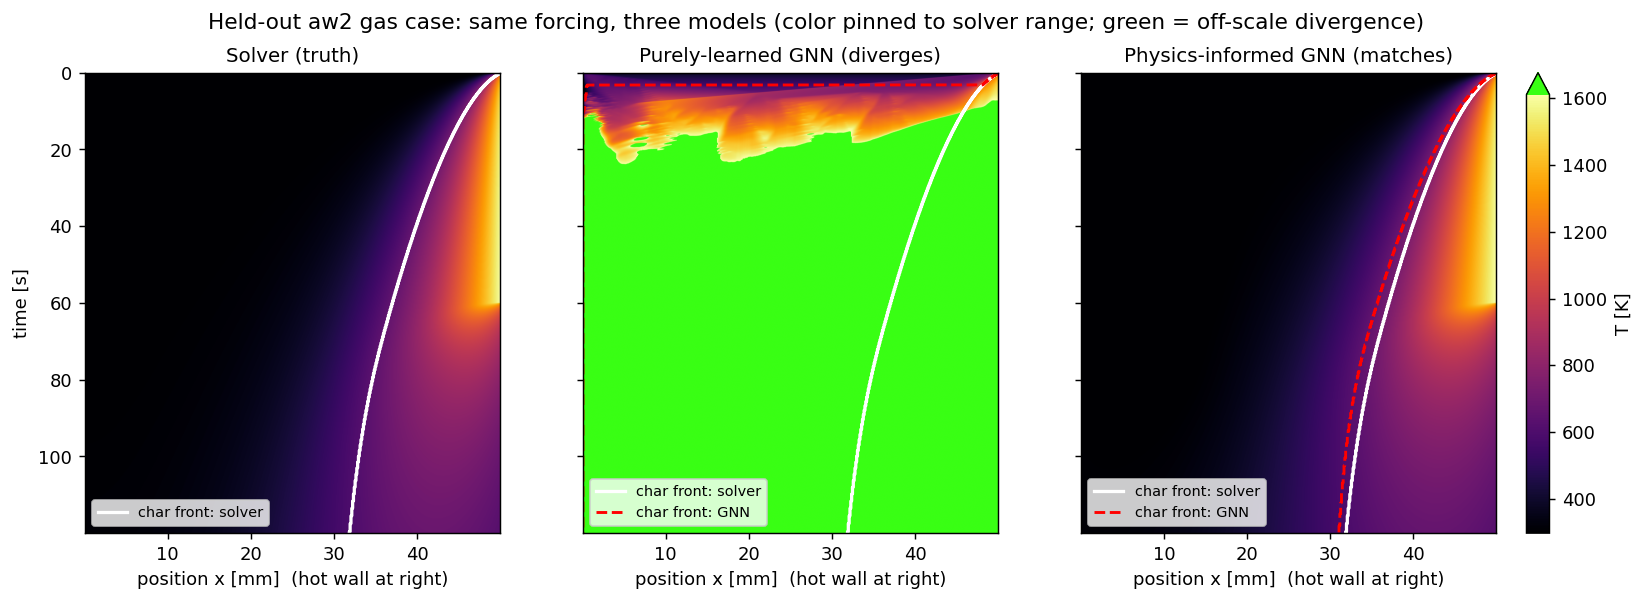
\includegraphics[width=\textwidth]{aw2_contrast_3map.png}
  \caption{Held-out \texttt{aw2} gas case, same forcing, three models. Space-time
  temperature with char-front curves (solver white, GNN red dashed). Left: Fortran
  solver truth. Center: the purely learned direct surrogate, which diverges past
  100{,}000~K and saturates off-scale (green), its char front collapsing to the back
  face. Right: the physics-informed conductance surrogate (twenty-four training
  forcings, real Arrhenius kinetics), which stays bounded to the solver's range and
  tracks the char front to about one millimeter. Color is pinned to the solver
  range, so any off-scale value is a divergence.}
  \label{fig:contrast}
\end{figure*}

\subsection{Wall Time}
The Fortran solver runs \texttt{aw2\_tc21} in about 3 minutes. The present
unoptimized Python implementation takes about 15.6 minutes, roughly five times
slower, as expected for interpreted array code against compiled Fortran. The
Python port's role is to generate verified training data and to be a readable
reference, not to be fast.

The surrogate is the fast path. On a held-out 120~s gas case its rollout takes about
92 seconds on a single GPU and about 100 seconds on a CPU, against about 925 seconds
for the same case in the Python solver. That is about ten times faster than the
Python solver and about twice as fast as the compiled Fortran. The advantage is
modest at this scale, and honestly so. The 1D mesh is small, so the fixed cost of
each network call is not amortized and a single GPU barely beats the CPU. The larger
gain this method targets is not exercised here. It comes from batching many design
cases through the GPU together and from the steeper per-step cost of the
higher-dimensional solvers the method is meant to extend to.

\section{Discussion}
The results establish three things. First, the multi-physics reference solver can
be reproduced faithfully in modular, readable Python, to machine precision on the
conduction-plus-pyrolysis case and to a small fraction of a kelvin on the full gas
case. That fidelity is what makes the solver usable as a data generator, since a
surrogate is only as trustworthy as the data it learns from. Second, a per-cell
message-passing GNN trained on that data is an accurate surrogate for the gas-off
case over a full rollout, including faithful tracking of the moving pyrolysis
front; its relative edge features give it the local information the physics uses,
and its weight sharing is what makes it mesh-native.

Third, the gas case marks where a purely learned model stops working and shows what
fixes it. A direct per-cell predictor diverges past 25{,}000~K on a held-out forcing
(Section~\ref{sec:aw2}). A conservative flux-form removes that catastrophic
divergence by construction, since a uniform field produces exactly zero change, but
it does not produce a faithful field. Across eight seeds some flux-form runs still
diverge, and the bounded ones are physically wrong, with a char front that reaches
the back face in most seeds (Section~\ref{sec:flux}). The fix is to stop asking the
network to learn the physics that is already known. We fix the conduction rate and
the Arrhenius pyrolysis to the reference solver, bound each update to a weighted
average of neighboring cells so it cannot overshoot, and leave the network only the
gas coupling to learn (Section~\ref{sec:physcond}). Embedding known physics into the
model rather than learning it is the principle behind physics-informed networks, and
here it is what keeps the rollout stable and physically consistent~\cite{cao2026}.
This physics-informed surrogate reproduces the held-out gas case to a 25~K mean
error, tracks the char front to about a millimeter, and does not degrade when the
training set grows from eight forcings to twenty-four. The lesson is about how much structure a surrogate needs.
The gas-off case is mild enough to learn end to end, while the stiff coupled gas
case needs its known physics built in. One weakness remains, a bias of about 50~K at
the hot surface near the flux cutoff, where the surrogate runs slightly hot. The
verification caution of Section~\ref{sec:aw1acc}, that a low domain-mean error can
hide an unphysical field, is exactly what the flux-form seed study showed, and it is
why we trust the char front rather than the mean.

\section{Future Work}
The physics-informed surrogate delivers a faithful and fast gas-case rollout
(Section~\ref{sec:physcond}), and several directions extend it. First, the surrogate
is a differentiable rollout, which opens gradient-based design optimization and
sensitivity analysis that the solver does not provide directly. Demonstrating a
design loop that uses those gradients is the natural next step. Second, the
conduction and pyrolysis rates are currently fixed to the solver. Relaxing them to
values learned around the known physical anchor would make the model more genuinely
learned while keeping it stable. Third, the surface bias near the flux cutoff is the
one remaining inaccuracy and is worth closing. Beyond the gas case, training across a
range of mesh resolutions would let one model run at resolutions it did not see. The
wall-time advantage should be measured across a design-relevant batch of
evaluations, where the method's real gain lies. Finally, the physics can be extended
with radiation, surface recession, and two- and three-dimensional meshes.

\section{Conclusion}
We re-implemented a coupled heat-conduction and pyrolysis heat-shield solver in
Python, verified it against the Fortran reference to machine precision on the
gas-off case and to 0.064~K on the full gas case, and trained a per-cell
message-passing GNN surrogate that reproduces a held-out gas-off rollout to 7.6~K.
On the full gas case a purely learned surrogate diverges, a failure we trace to a
fixed-step state-delta formulation and a stiff aerothermal transient. Building the
known physics into the surrogate fixes it. Fixing the conduction rate and the
Arrhenius pyrolysis to the reference solver, bounding each update so it cannot blow
up, and learning only the residual gas coupling yields a surrogate that reproduces a
held-out gas case to a 25~K mean error, tracks the char front to about a millimeter,
and runs about ten times faster than the Python solver. The result is a lesson about
structure. A mild problem can be learned end to end, while a stiff coupled problem
needs its known physics built in. Mesh-resolution generalization, a demonstrated
design-optimization loop using the surrogate's gradients, and extension to higher
dimensions are the next steps.

\section*{Acknowledgment}
add

\bibliographystyle{IEEEtran}
\bibliography{heat_gnn_refs}

\end{document}
